\documentclass{book}
\usepackage[utf8]{inputenc}
\usepackage[english,ngerman]{babel}
\usepackage{datetime}
\usepackage{graphicx}
\usepackage{xspace}
\usepackage{hyperref}
\usepackage{listings}
\usepackage{float}
\usepackage{keystroke}
\usepackage{xcolor}
\usepackage{enumitem}
\usepackage{wrapfig}
\usepackage{amsmath}
\usepackage{tikz}
\usetikzlibrary{arrows,shapes,positioning}
\usetikzlibrary{calc,decorations.markings}

\newdateformat{germanDate}{\twodigit{\THEDAY}.\twodigit{\THEMONTH}.\THEYEAR}

% eigene Commands
\newcommand{\sketchup}{\texttt{SketchUp}\xspace}
\newcommand{\rubyXL}{\texttt{rubyXL}\xspace}
\newcommand{\inifile}{\texttt{inifile}\xspace}
\newcommand{\version}{Version v1.1}
\newcommand{\robersexcelconvert}{\texttt{RobersExcelConvert}\xspace}
\newcommand{\assisttool}{\texttt{Translations Organizer}\xspace}
\newcommand{\hinweis}[1]{\newline \textbf{Hinweis}: #1 \newline}
\newcommand{\green}[1]{\color{green!50!black}#1\color{black}\xspace}
\newcommand{\red}[1]{\color{red}#1\color{black}\xspace}
\newcommand{\orange}[1]{\color{orange}#1\color{black}\xspace}

% Define block styles
\tikzstyle{decision} = [diamond, draw, top color=white, bottom color=blue!20 text width=4.5em, text badly centered, node distance=3cm, inner sep=0pt]
\tikzstyle{block} = [rectangle, draw, top color=white, bottom color=blue!20, text width=5em, text centered, rounded corners, minimum height=4em]
\tikzstyle{line} = [draw, -latex']
\tikzstyle{cloud} = [draw, ellipse,fill=red!20, node distance=3cm, minimum height=2em]

\begin{document}
	
	\begin{titlepage}
	\centering
	
\includegraphics{pics/sketchup-icon}\par\vspace{1cm}
	%		{\scshape\LARGE Columbidae University \par}
	
	\vspace{1.5cm}
	{\huge\bfseries Robers' Excel Convert\par}
	\vspace{1cm}
	{\scshape\Large - Anleitung -\par}
	\vspace{2cm}
	{\Large\itshape Timo Bergerbusch\par}
	\vfill
	im Auftrag von:\par
	Max Robers
	
	\vfill
	
	{\large \germanDate\today\par}
\end{titlepage}
	
	\tableofcontents
	\chapter{Das RobersExcelConvert-Plugin} \label{RobersExcelConvert}
		Für die \textit{Paletten Robers GmbH} wurde nach einer Lösung gesucht um den Aufwand für die Zeichnungen von zuweilen Standard Kisten vom Typ \textit{CF-015} zu zeichnen. Durch Änderung der Länge einer bereits gezeichneten Kiste ist der Aufbau analog, allerdings ist der manuelle Aufwand eine Zeichnung fehlerfrei zu ändern ist wesentlich höher als man am Anfang vermuten kann.\\
		Um den Zeichenaufwand zu minimieren und einem Kunden kurzfristig eine Zeichnung bieten zu können soll der Prozess der Zeichnung anhand der gegebenen Stückliste in aus einer exogenen Excel-Datei automatisiert werden. Jede Stückliste nach dem Format, welches bis zu einem gewissen Grad angepasst werden kann, kann von der gelieferten Implementierung gezeichnet werden.\\
		\\
		Der generelle Ablauf der einzelnen Programm teile ist im folgenden erklärt. Insgesamt lässt sich der Programm Ablauf in 3 Teile aufteilen lassen, wie es auch in Abbildung \ref{fig:general Flow} zu sehen ist:
		\begin{enumerate}
			\item Das \assisttool aufrufen
			\item eine Excel-Datei einlesen und interpretieren
			\item die Excel dem \robersexcelconvert-Plugin übergeben
		\end{enumerate}
		
		\begin{figure}[H]
			\begin{tikzpicture}[node distance = 8cm, auto] 
				\node [block, minimum width = 3cm] (assist) {\assisttool};
				\node [block, minimum width = 3cm, right of =  assist] (sketchup) {\sketchup};
				\path [line] (assist) -- node {gelesene Excel} (sketchup);
			\end{tikzpicture}
			\caption{Der generelle Ablauf}
			\label{fig:general Flow}
		\end{figure}
		Jedes dieser Teile kann weiter aufgebrochen werden im Sinne des Ablaufs der Aufgaben, welche es jeweils zu bewältigen geht.
		
		\section{Der \assisttool Ablauf}
			
			Ab Version v1.1 wird jegliche Form der Berechnung und Identifizierung im \assisttool ausgeführt. Demnach ist die Menge der Aufgaben des \assisttool relativ groß. Ein Ablauf-Diagramm ist zu sehen in Abbildung \ref{fig:assist flow}.
			\begin{figure}
				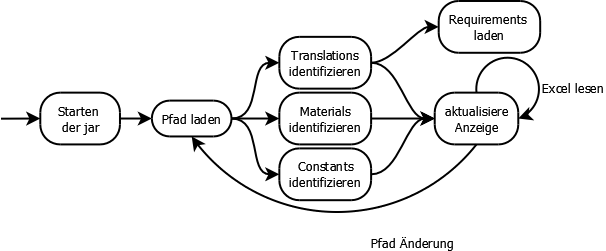
\includegraphics[scale=0.4]{diagramms/translationsOrganizer-ablauf.png}
				\caption{Der generelle Ablauf}
				\label{fig:assist flow}
			\end{figure}
			Es wird die Anwendung gestartet basierend auf dem gesetzten \texttt{Default}-Pfad, welche den SketchUp Ordner der Arbeitsumgebung erwartet. Im Standard Fall wird es \begin{center}
				\texttt{C:\textbackslash Users\textbackslash Timo Bergerbusch\textbackslash AppData\textbackslash Roaming\textbackslash SketchUp\textbackslash SketchUp 2018\textbackslash SketchUp}
			\end{center}.
			\hinweis{Dies ist \underline{nicht} das Installationsverzeichnis}
			Anschließend werden dort nach den drei folgenden Dateien gesucht:
				\begin{enumerate}
					\item \texttt{translations.ini}: alle gespeicherten \hyperref[Translation]{Translations}
					\item \texttt{materials.ini}: alle gespeicherten \hyperref[Material]{Material Zuweisungen}
					\item \texttt{constants.ini}: alle gespeicherten \hyperref[excel konstanten]{Konstanten}
				\end{enumerate}
			Basierend auf den Material Zuweisungen und den dort verwendeten Texturen werden die Requirements geladen, welche dann im \hyperref[semantic check]{Semantik Check} auf Verfügbarkeit überprüft werden. Sobald im \hyperref[semantic check]{Semantik Check} der Pfad geändert wird aktualisieren sich die Translations und Material Zuweisungen basierend auf dem neuen Pfad.
			\hinweis{in Version v1.1 bleiben die Requirements gleich}
			
			\begin{figure}
				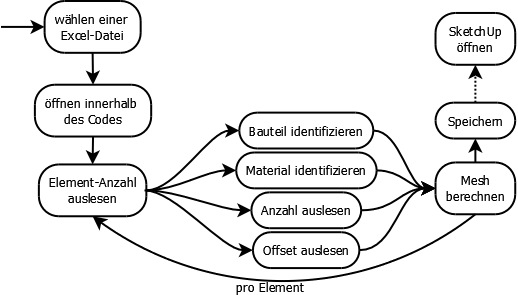
\includegraphics[scale=0.4]{diagramms/excelRead-ablauf.png}
				\caption{Der Ablauf beim einlesen einer Excel-Datei}
				\label{fig:excelRead flow}
			\end{figure}
			
			
		\section{Der Ablauf einer gelesenen Excel}
			Der Ablauf des \hyperref[excelread]{Einlesens einer Excel} ist abgebildet in Abbildung \ref{fig:excelRead flow}. Nachdem eine Datei gewählt wurde und die entsprechende Java-Bibliothek die Datei eingelesen hat, was teilweise 1 oder 2 Sekunden dauern kann wird in der Excel, welche den Aufbau hat welcher in \ref{excel} vorgestellt wird, basierend auf der Spalte \textit{Säge Art.} gezählt wie viele Elemente in der Stückliste aufgelistet sind. Ein Element ist eine gesamte Reihe mit allen relevanten Informationen nach der folgenden Aufteilung:\\
			\begin{figure}
				\centering
				\begin{tabular}{r | l}
					Teil von & Dazugehörige Spalten \\
					Bauteil & Bezeichnung, Bauteil, Länge, Breite, Höhe \\
					Anzahl & Anz. \\
					Material & Materialgruppe, Werkstoff \\
					Koordinaten & -nicht sichtbar gelistet-
				\end{tabular}
				\caption{Die Aufteilung der Spalten in teilerfremde Menge}
				\label{table:sets}
			\end{figure}
			\subsection{Bauteil identifizieren}\label{bauteil ident}
				Das Bauteil wird basierend auf den zwei Elementen Bezeichnung und Bauteil aus der in Tabelle \ref{table:sets} definierte Teilmenge Bauteil, identifiziert. Dies passiert in einem zwei-stufigen Prozess, wobei zuerst nach dem Bezeichnungs-Kürzel und anschließend nach einem Teil-String im Bauteil geprüft wird. Anschließend werden Länge, Breite und Höhe basierend auf der gefundenen Translation auf die X, Y und Z-Achse gemappt. \\
				\hinweis{Falls keine Translation gefunden werden kann wird das Mapping $$h: \text{Länge}\rightarrow\text{X-Achse},\text{Breite}\rightarrow\text{Y-Achse},\text{Höhe}\rightarrow\text{Z-Achse} $$ verwendet. In der Übersicht wird dann das Kürzel \texttt{default} genutzt und es wird automatisch als \texttt{daneben} gekennzeichnet}
			\subsection{Material identifizieren}
				Die Material Zuweisung wird analog zu der Bauteil Identifizierung in \ref{bauteil ident} berechnet basierend auf der Materialgruppe und Werkstoff. Demnach werden die Texturen ausgewählt die auf die jeweilige Seite gelegt werden
				\hinweis{Falls keine Material Zuweisung gefunden werden kann wird auf jeder Seite eine sog. \texttt{errorTexture} genutzt. In der Übersicht wird dann das Kürzel \texttt{default} genutzt und es wird automatisch als \texttt{daneben} gekennzeichnet}
			\subsection{Anzahl und Offset}
				Die Anzahl, welche beschreibt wie oft ein Maß-gleiches Bauteil gezeichnet werden soll, und der Offset, welcher genutzt wird um das Bauteil an einer speziellen Stelle zu zeichnen um direkt eine gesamte Kiste in der richtigen Konfiguration zu zeichnen, werden aus der Excel direkt abgelesen ohne weitere Interpretation. Dabei wir der Offset bei einer \hyperref[excel konstanten]{Konstanten} startend abgelesen nach dem Schema:
				An der Konstanten-Koordinate $c_{start}$ schaue nach dem X-Achsen-Offset $x_0$, eine Spalte weiter rechts nach dem Y-Achsen-Offset $y_0$ und noch eine Spalte weiter nach dem Z-Achsen-Offset $z_0$. Falls die Anzahl $a > 1$ ist müssen weitere Koordinaten gefunden werden. Demnach werden diese in der selben Zeile in Spalte $c_{start}+3$ gesucht und heißen demnach $x_1, y_1$ und $z_1$. Analog für alle weiteren Elemente. 
				
				\begin{figure}
					\centering
					\begin{tikzpicture}[square/.style={regular polygon,regular polygon sides=4}, every node/.style = {square, draw, minimum width = 1.4cm}]
						\node at (0,0) {3};
						\node at (1,0) {7};
						\node at (2,0) {-7};
						
						\node at (3,0) {6};
						\node at (4,0) {8};
						\node at (5,0) {9};
						
						\node at (6,0) {6};
						\node at (7,0) {1};
						\node at (8,0) {-5};
						
						\node at (9,0) {-3};
						\node at (10,0) {6};
						\node at (11,0) {2};
					\end{tikzpicture}\\
					\vspace*{1cm}
					
					\begin{tabular}{r|c|c|c|c}
						Bauteil Nr. & 1 & 2 & 3 & 4 \\\hline
						Variablen & $(x_1, y_1, z_1)$ & $(x_2, y_2, z_2)$ & $(x_3, y_3, z_3)$ & $(x_4, y_4, z_4)$ \\ \hline
						Werte & $(3,7,-7)$ & $(6,8,9)$ & $(6,1,-5)$& $(-3,6,2)$ 
					\end{tabular}
					\caption{Beispiel Koordinaten für ein Element mit einer Anzahl von 4}
					\label{bsp:koords}
				\end{figure}
			
			
			Im Anschluss zum identifizieren des gesamten Elements kann das Bauteil berechnet werden und es kann in einer Datei gespeichert werden, welche dann weiter gegeben wird an das \robersexcelconvert-Plugin, welches beim Start von \sketchup ausgeführt wird.\\
			Zusätzlich kann automatisch \sketchup geöffnet werden.
			\section{Ablauf bei \sketchup}
				\begin{figure}[H]
					\includegraphics[scale=0.4]{diagramms/sketchup-ablauf.png}
					\caption{Der Ablauf innerhalb von \sketchup}
					\label{fig:sketchup flow}
				\end{figure}
				Innerhalb von \sketchup wird beim Starten durch den \assisttool zuerst eine leere Zeichnung geöffnet. Dort findet sich ein Button in der Toolbar, mittels welchem die vom \assisttool gespeicherten Elemente gezeichnet werden können. Dabei wird die Datei mit den Elementen gelöscht. Falls man etwas an den zum Beispiel Offset-Koordinaten geändert wurden kann im \assisttool auf \textit{Speichern} genutzt werden und dann im \sketchup Fenster durch das nutzen des Buttons aktualisiert werden. Dabei werden die vorherigen gezeichneten Elemente gelöscht und die neuen werden neu gezeichnet.
	\chapter{Voraussetzungen}
		\section{\sketchup Version} \label{sketchup version}
			Die \sketchup-Version ist ab Version v1.1 nicht weiter relevant. Als Gems wird nur noch das \inifile-Gem benötigt, welches auch mit älteren \sketchup Versionen kompatibel ist.
		\section{Ruby Konsole} \label{Ruby Konsole}
			Die Ruby Konsole ist ein essentieller Bestandteil des \robersexcelconvert-Gems, da durch sie wichtige Ausgaben getätigt werden. Zudem kann dort geprüft werden, ob das Gem erfolgreich installiert wurde und somit die angepriesene Leistung erbringen kann.\\
			Die Konsole kann geöffnet werden durch die folgenden einfachen Schritte:
				\begin{enumerate}
					\item \sketchup starten:
						Um die Konsole zu öffnen muss natürlich anfangs \sketchup gestartet werden.
					\item Die Ruby Konsole öffnen:
						Anschließend klicken Sie in dem geöffneten auf:
						\begin{figure}[H]
							\centering
							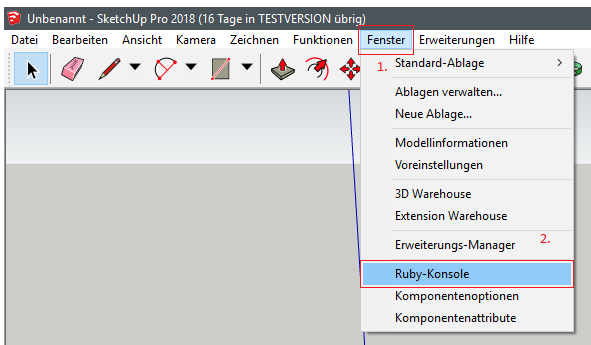
\includegraphics[scale=0.6]{pics/Ruby-Konsole-oeffnen.png}\\
							\texttt{Fenster $\rightarrow$ Ruby Konsole}							
						\end{figure}
						Anschließend sollte sich die Ruby Konsole öffnen. Dort kann man unter anderem nun den \hyperref[Funktionstest]{Funktionstest} durchführen.
				\end{enumerate}
		\section{Toolbar anzeigen}
			Durch einen Rechtsklick auf die allgemeine Toolbar können die Erweiterungen gewählt werden, welche sichtbar sein sollen. Durch das auswählen der \texttt{Robers Excel Convert}-Option wird die benötigte Option Sichtbar. \\
			Es kann vorkommen, dass die Toolbar als einzelnes kleines Icon als ein Fenster geöffnet wird. Diese kann durch Drag-and-Drop in die normale Toolbar eingelassen werden.
			\begin{figure}[H]
				\centering
				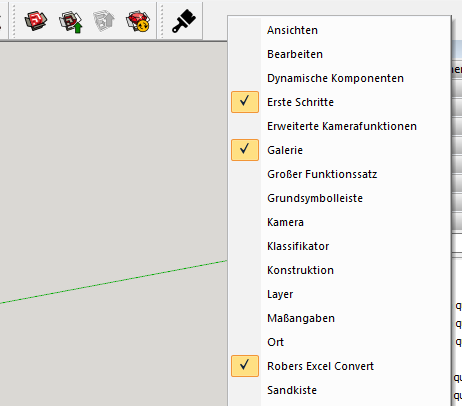
\includegraphics[scale=0.4]{pics/toolbar.png}
				\caption{Das Menü um die Toolbar anzeigen zu lassen}
				\label{toolbar}
			\end{figure}
		\section{\sketchup - Gliederung}
			Die Gliederung ist eine \sketchup-interne Liste, welche alle Bauteile auflistet. Dies ist nützlich, da bei dem Zeichnen der Stückliste alle Elemente mit dem in der \hyperref[excel]{Excel-Datei} unter der Spalte \textit{Bauteil} beschriebenen Namen genauso benannt in \sketchup gezeichnet werden. So kann zu jedem gezeichneten Bauteil, welches vielleicht eine falsche oder falsch konfigurierte \hyperref[Translation]{Translation} nutzt, per Name direkt erkannt wird. So kann in der Bauteilliste %TODO link
			das entsprechende \textit{Kürzel} der \hyperref[Translation]{Translation} direkt abgelesen werden.\\
			Die Gliederung kann durch die folgenden Schritte aktiviert werden:
			\begin{figure}[H]
				\centering
				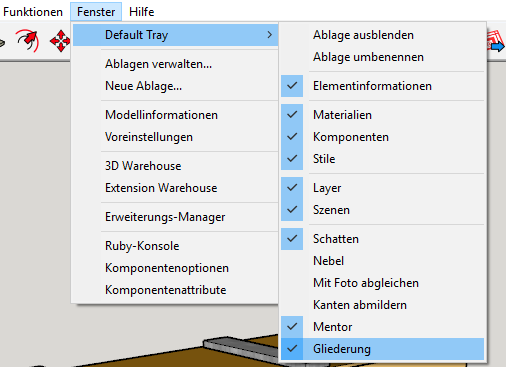
\includegraphics[scale=0.6]{pics/Gliederung.png}\\
				\texttt{Fenster $\rightarrow$ Default Tray $\rightarrow$ Gliederung}							
			\end{figure}
			Sobald die \textit{Gliederung}-Option aktiviert wurde ist im \textit{Default Tray} Fenster die gewünschte Auflistung zu finden. \\
			Ein Beispiel dafür ist zu sehen in Abbildung \ref{Gliederung Beispiel}.
			\begin{figure}[H]
				\centering
				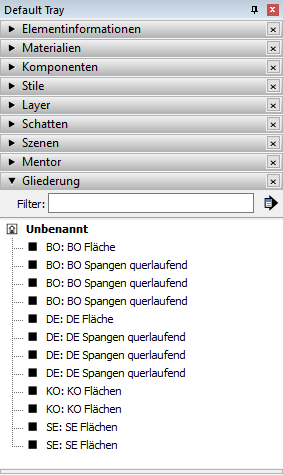
\includegraphics[scale=0.6]{pics/Gliederung-Beispiel.png}
				\caption{Beispiel für eine Gliederung von Bauteilen in der \textit{Gliederung}}
				\label{Gliederung Beispiel}
			\end{figure}
			
		\section{Bibliotheken installieren} \label{Installation}
			Im Laufe des Programms wird eine Bibliotheken verwendet: inifile\\\label{inifile}
				Das \inifile-Gem wird benötigt um die \hyperref[Translations]{Translations} zu speichern und zu verwalten. Mittels diesem Gem werden *.ini-Dateien gelesen, geschrieben und gespeichert. Analog zum \rubyXL-Gem kann das Gem in der \hyperref[Ruby Konsole]{Ruby Konsole} installiert werden via:
				\lstinputlisting[xleftmargin=0.1\textwidth,xrightmargin=0.2\textwidth]{listings/installGem-inifile.txt}
				Das \inifile-Gem braucht keine weiteren Gems.
			\begin{figure}[H]
				\centering
				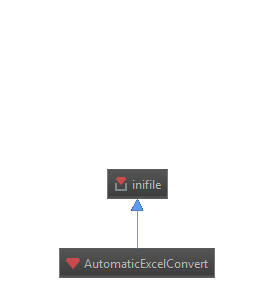
\includegraphics[scale=0.6]{pics/Gemdependency-full.png}
				\caption{Der Abhängigkeitsgraph der Gems}
				\label{Abhaengigkeitsgraph}
			\end{figure}
		\section{Gem einfügen}
			Das \robersexcelconvert-Gem muss um mit \sketchup funktionieren zu können in den richtigen Ordner kopiert werden. 
			Dazu muss der \glqq Plugins \grqq-Ordner geöffnet und die angegebene Datei und Ordner kopiert werden.
			Dies ist notwendig, damit das \robersexcelconvert-Gem direkt beim Start von \sketchup geladen wird und verwendet werden kann.
			\subsubsection{Plugins-Ordner}
				Der Plugins-Ordner ist erreichbar über die folgenden Schritte:
				\begin{enumerate}
					\item Windows Explorer öffnen:\\
						\begin{figure}[H]
							\centering
							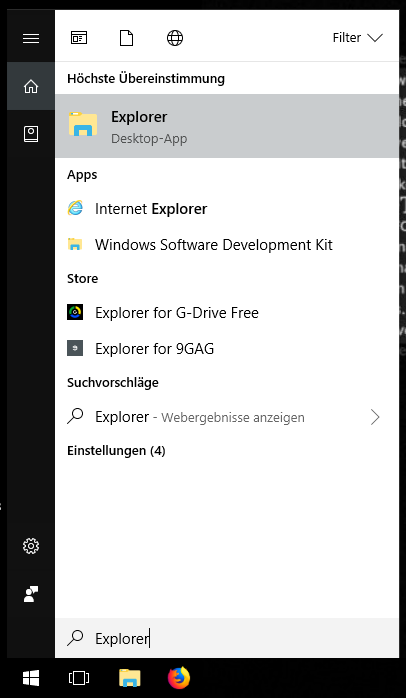
\includegraphics[scale=0.5]{pics/plugins-ordner/Explorer-oeffnen.png}
							\caption{Der Explorer wird mittels Starmenü geöffnet}
						\end{figure}
						Öffnen Sie den Explorer mittels des Windows-Startmenüs oder der Tastenkombination: \keystroke{Win}+\keystroke{E}
						\label{explorer oeffnen}
					\item Zur Roaming navigieren:\\
						\begin{figure}[H]
							\centering
							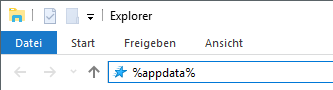
\includegraphics[scale=0.6]{pics/plugins-ordner/appdata-eingeben.png}
							\caption{In die Adresszeile wird die angegebene Text direkt eingefügt}
						\end{figure}						
						Navigieren Sie zur Roaming des Benutzers. Dies ist möglich durch die Eingabe von:\texttt{\%appdata\%} in die Adresszeile. Alternativ kann man den absoluten Pfad angeben, welcher meist wie folgt aussieht:
						\lstinputlisting[xleftmargin=0.1\textwidth,xrightmargin=0.2\textwidth]{listings/roamingpath.txt}
						wobei \texttt{BENUTZERNAME} durch den Namen des aktuellen Windows Nutzers ersetzt werden muss.\\
						\underline{Wichtig}: Es müssen versteckte Ordner angezeigt werden um manuell zum Roaming Ordner zu navigieren.
					\item Zum Plugins Ordner navigieren:
						\begin{figure}[H]
							\centering
							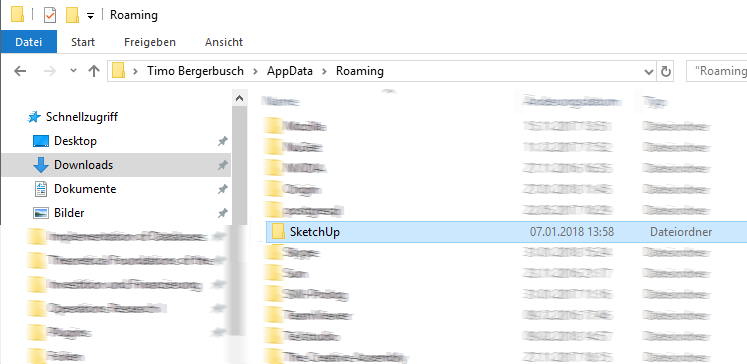
\includegraphics[scale=0.6]{pics/plugins-ordner/Sketchup-Ordner.png}
							\caption{Der \sketchup-Ordner in der Roaming}
						\end{figure}
						In dem nun geöffneten Roaming suche Sie nach dem Ordner mit Namen: \sketchup .
						Innerhalb von diesem Ordner öffnen Sie die folgende Ordnerstruktur: 
						\lstinputlisting[xleftmargin=0.1\textwidth,xrightmargin=0.2\textwidth]{listings/pluginspath.txt}
						Dies ist der Ordner in welchen nun mit dem folgenden Schritt das \robersexcelconvert-Gem eingefügt werden sollte.
					\item Kopieren:
						\begin{figure}[H]
							\centering
							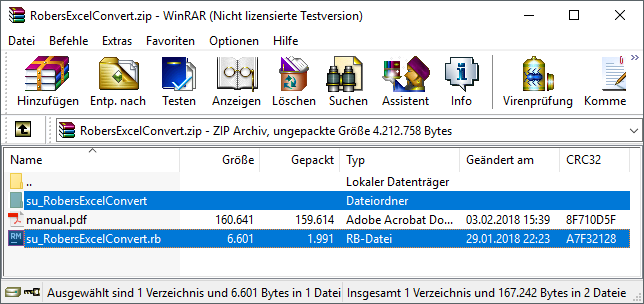
\includegraphics[scale=0.6]{pics/plugins-ordner/zip-datei.png}
							\caption{Die markierten zu kopierenden Datei und Ordner}
						\end{figure}
						Kopieren sie die markierten Datei \texttt{su\_RobersExcelConvert.rb} und den markierten Ordner \texttt{su\_RobersExcelConvert} in den soeben geöffneten \texttt{Plugins}-Ordner.
						\begin{figure}[H]
							\centering
							\includegraphics[scale=0.6]{pics/plugins-ordner/plugins-ordner.png}
							\caption{Der Plugins-Ordner nach dem einfügen der Datei und des Ordners}
						\end{figure}
				\end{enumerate}
		\section{Funktionstest}\label{Funktionstest}
			Wenn das \robersexcelconvert-Gem korrekt eingefügt wurde und das Gem wie gewünscht funktioniert kann per \hyperref[Ruby Konsole]{Ruby Konsole} getestet werden, ob das Plugin funktioniert\\
			Dazu muss in der Konsole der folgende Befehl eingegeben werden:
			\lstinputlisting[xleftmargin=0.2\textwidth,xrightmargin=0.2\textwidth]{listings/funktionstest.txt}
			Dies gibt bei korrekter Integration des Plugins: \texttt{Successfully loaded.} zurück. Ein Beispiel dafür ist zusehen in \ref{funktionstest-success}\\
			
			\begin{figure}[H]
				\centering
				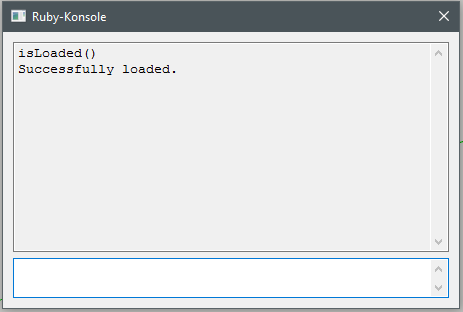
\includegraphics[scale=0.6]{pics/funktionstest.png}
				\label{funktionstest-success}
			\end{figure}
			
			Ansonsten wird ein Fehler zurück gegeben, dass die Methode nicht bekannt ist und somit das Plugin nicht richtig eingebunden wurde. In einem solchen Fall sollte das Tool: \assisttool genutzt werden, um den Grund des nicht erfolgreichen Funktionstest festzustellen.
	\chapter{\assisttool}\label{assisttool}
		Der \assisttool ist ab Version v1.1 die Hauptapplikation. In ihr wird jedes Bauteil identifiziert, die \hyperref[Translation]{Translation} und die \hyperref[Material]{Materialen} davon abgeleitet und schlussendlich dem \robersexcelconvert-Plugin übergeben. Zudem kann ab Version v1.1 \sketchup durch das \assisttool gestartet und simultan genutzt werden. So ist es möglich eine Stückliste quasi-live zu bearbeiten. Beispiele für eine solche quasi-live Bearbeitung sind gelistet in %TODO link
		. Das \assisttool verfügt über die im folgenden weiter ausgeführten Funktionen:
			\begin{itemize}
				\item eine Excel auslesen und zeichnen lassen
				\item Semantik-Check
				\item Translations bearbeiten
				\item Materialzuweisungen bearbeiten
				\item Konstanten bearbeiten
			\end{itemize}
		\section{Excel auslesen und zeichnen}\label{excelread}
			Eine Excel-Datei in dem Format, wie es zum Stand des 12.04.2018 vorlag, kann ausgelesen und anschließend in \sketchup gezeichnet werden.
			\begin{figure}
				\centering
				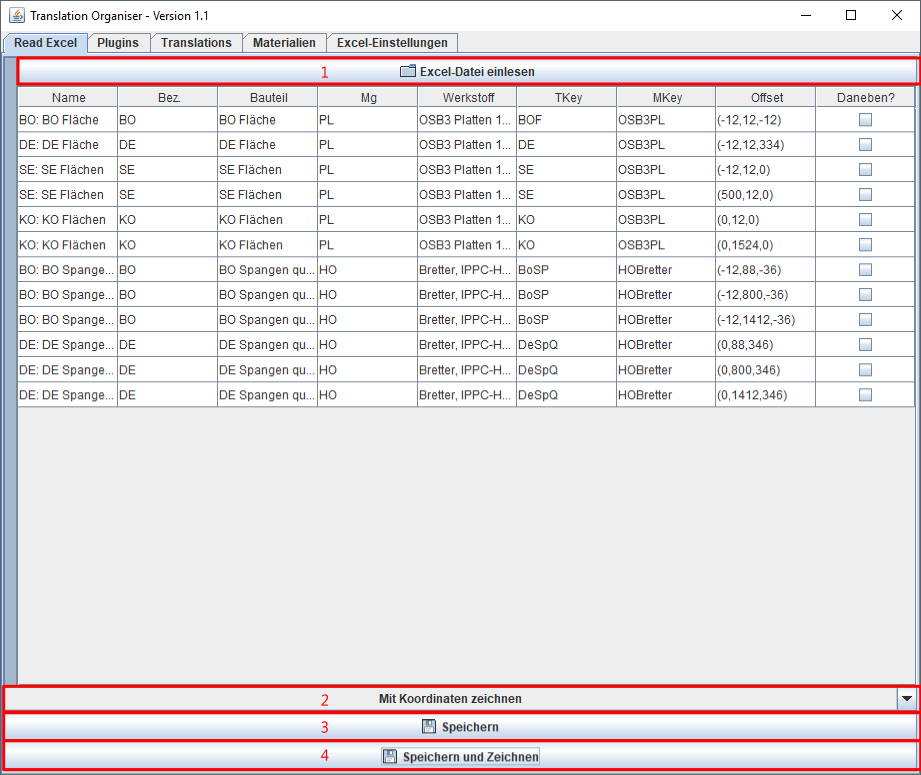
\includegraphics[scale=0.48]{pics/assisttool/readExcel.png}
				\caption{Die Oberfläche um Dateien einzulesen und zu zeichnen}
				\label{fig:read Excel}
			\end{figure}
			\subsection{Excel auswählen}
				Eine Excel kann ausgewählt werden durch die Schaltfläche mit der Nummer 1 in Abbildung \ref{fig:read Excel}. Mit dem anschließenden Datei-Öffnen-Dialog kann die zu öffnende Excel-Datei ausgewählt werden. Diese wird dann durch die \hyperref[REC - Ablauf]{Abarbeitungsvorschrift} geschleift und anschließend in der Tabelle aufgelistet. 
			\subsubsection{Elemente bearbeiten} \label{element bearbeiten}
				Die aufgelisteten Elemente können in Version v1.1 können in der Spalte der Offset-Koordinaten manipuliert werden. Die Offset-Koordinaten beschreiben einen Vektor vom Ursprung aus, um welchen das Bauteil verschoben wird. Sie beschreibt die Koordinate der "unteren linken Ecke". Von diesem wird auf der X,Y und Z-Achse der positive Wert abgetragen.\\
				Die Koordinate kann manuell auf einen anderen Wert gesetzt werden, durch einen Doppelklick auf die Zelle und das Eintragen der neuen Werte. Nach dem ändern wird ein Check durch eine Regulären Ausdruck gemacht ob der Ausdruck die folgende Form hat:
					$$ ( \text{X-Offset}, \text{Y-Offset}, \text{Z-Offset})$$
				wobei X/Y/Z-Offset ein ganzzahliger Wert ist.\\
				Falls die Eingabe nicht die gewünschte Form hat wird der vorherige Wert unverändert gelassen.\\
				Zudem ist es möglich durch das Anwählen der \textit{CheckBox} ein Bauteil neben der eigentlichen Kiste zu zeichnen. Die Definition von \glqq daneben \grqq ist gegeben durch die Konstanten-Werte, welche unter dem \hyperref[excel konstanten]{Excel-Einstellungen-Tab} zu finden ist.\\
				Weiter ist es möglich die Bauteile einmal als Kiste also mit den Koordinaten zu zeichnen, oder alle ähnlichen Elemente nebeneinander und unterschiedliche Elemente übereinander zu zeichnen um diese manuell zu ändern. Dazu nutzt man die Schaltfläche Nummer 2 in Abbildung \ref{fig:read Excel}.
			\subsection{Speichern}
				Das Speichern der Tabelle ist nötig, um es an das \robersexcelconvert-Plugin weiter zu geben. Es wird eine Datei angelegt im Verzeichnis wo auch die Ruby-Dateien erwartet werden. Der einzige Unterschied zwischen der Schaltfläche Nummer 3 und 4 in Abbildung \ref{fig:read Excel} ist, ob \sketchup geöffnet werden soll oder nur die Datei geschrieben. So ist die quasi-live Nutzung möglich. 
			\subsection{Quasi-Live Nutzung}
				Nachdem eine Excel-Datei eingelesen wurde und einmal die Schaltfläche Nummer 4 aus Abbildung \ref{fig:read Excel} genutzt wurde hat man den \assisttool und eine \sketchup-Instanz offen. Nun kann durch das Nutzen der Schaltfläche Nummer 3 in Abbildung \ref{fig:read Excel} die Datei mit den z.B. veränderten Koordinaten gespeichert werden und durch die Schaltfläche in \sketchup direkt neu gezeichnet werden ohne \sketchup neu zu starten.\\
				Im Falle der Änderung von Translations oder Material-Texturen kann auch dies genutzt werden und die Änderung eingetragen, \underline{ohne} \sketchup neu zu starten. Beispiele zu der Nutzung sind gegeben in %TODO Beispiele anfertigen
		\section{Semantik-Check}\label{semantic check}
			Der Semantik-Check des \assisttool s kann genutzt werden um die Installation zu überprüfen. Es werden unter anderem die Bibliotheken geprüft. 
			\hinweis{Für die Bibliotheken werden in Version v0.2 nur die exakten Versionen der Bibliotheken getestet. Eine Erkennung unter der Bedingung einer min. so aktuellen Version soll in den laufenden Updates kommen.}
			Der Reiter des Semantik-Checks besteht aus den unter \hyperref[fig:semantik check]{Abbildung \ref{fig:semantik check}} gelisteten Elementen.				
			
			\begin{figure}
				\centering
				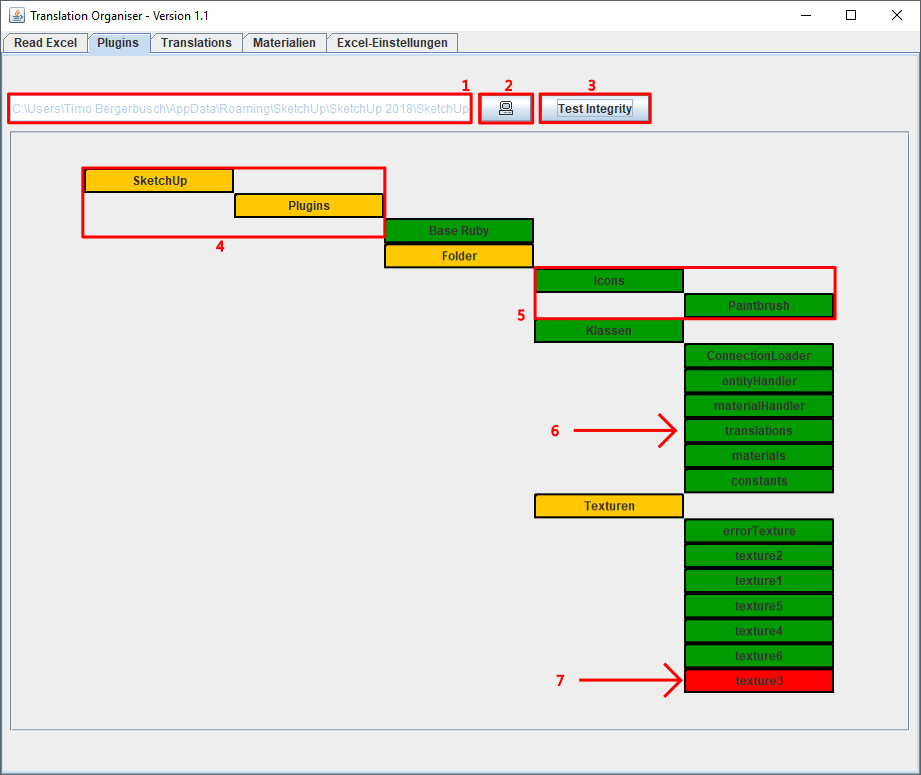
\includegraphics[scale=0.48]{pics/assisttool/semantik-check.png}
				\caption{Die Oberfläche des Semantik-Checks}
				\label{fig:semantik check}
			\end{figure}
		
			Das Interface unterteilt sich in die folgenden Elemente:
			\begin{enumerate}
				\item Dieses Textfeld wird genutzt um den Pfad anzugeben, welcher die folgenden Elemente beinhalten sollen. Dieser Ordner sollte der \sketchup-Ordner sein, in welchen unter \ref{Installation} die Installation durchgeführt wurde. \hinweis{\underline{NICHT} der Plugins-Ordner}
				\item Diese Schaltfläche öffnet die Windows \glqq Datei-Öffnen \grqq-Dialog und erleichtert die Suche des gewünschten Ordners. Es kann der Ordner ausgewählt werden und mittels "Öffnen" wird dieser übernommen.
				\item Diese Schaltfläche führt den Test aus. Sie geht von dem unter 1. gewählten Pfad aus und überprüft rekursiv ob die geforderten Elemente vorhanden sind. 
				\item Ein solcher Sprung stellt eine sog. Erbschafts-Beziehung dar. Dies bedeutet im Beispiel, dass \glqq Plugins \grqq innerhalb von \glqq SketchUp\grqq sich befindet. Demnach ist \glqq SketchUp\grqq ein Ordner. 
				\item Ein solcher Spring, indem einmal zur Seite gegangen wird, symbolisiert, dass \glqq Icons\grqq ein Ordner ist. Weiterhin haben die dem \glqq Icons\grqq -Ordner untergeordneten Elemente keine weiteren Teilelemente, was bedeutet, dass es Dateien sind.
				\item Diese Datei wurde erfolgreich geladen. Die bedeutet sie befindet sich im gewünschten Ordner mit der gewünschten Bezeichnung. Solche Elemente werden mit \green{Grün} markiert.
				\item Diese Datei wurde nicht angetroffen. Dies kann bedeuten, dass die Datei nicht vorhanden ist, oder einen anderen Namen trägt. \hinweis{Die Endung ist auch entscheidend. Texturen werden in Version v.02 \underline{ausschließlich} im \glqq jpg \grqq-Format akzeptiert.}
				Solche Elemente bekommen die Farbe \red{Rot}.
				\item Elemente welche in der Ordner-Hierarchie übergeordnet sind, werden falls ein Element damit nicht korrekt geladen wurde mit der Farbe \orange{Orange} markiert. Dies bedeutet, dass der Ordner zwar existiert, aber etwas innerhalb dieses Ordners nicht korrekt ist. 
			\end{enumerate}			
		
		\section{Translations} \label{Translation}
			Die Translations bestimmen, welche Werte der in der Excel eingetragenen Elemente (Länge, Breite, Höhe) auf welche der 3 Achsen projiziert werden soll. Eine Translation besteht aus den folgenden Elementen:
			\begin{itemize}
				\setlength{\itemindent}{1cm}
				\item[Name:] Der Name, welcher für das Element verwendet werden soll. Er dient allein der Leserlichkeit bei Ausgaben
				\item[Key:] Der Key, welcher genutzt wird um ein Element innerhalb der Datei eindeutig zu identifizieren. Keine zwei Translations dürfen den selben Key haben.
				\item[Kürzel:] Das Kürzel ist die Abkürzung die in der \glqq Kürzel\grqq -Spalte innerhalb der Excel-Datei verwendet wird (siehe auch \hyperref[excel]{\ref{excel}}). Anhand dieser kann weiter auf dem Bauteil basierend identifiziert werden, welches Konstrukt es ist.
				\item[Bauteil:] Das Bauteil ist die zweite Stufe der Identifizierung eines Konstruktes. Basierend auf dem Eintrag innerhalb der Excel in der Spalte \glqq Bauteil \grqq wird das \underline{erste} Element ausgesucht, welches die hier eingetragene Zeichenkette beinhaltet.
				\hinweis{Falls diese Spalte für eine Zelle leer ist, können alle Konstrukte, welche das zugehörige Kürzel haben als geeignet angesehen}
				\item[X-Achse:] Beschreibt, welche Einheit auf der X-Achse abgetragen werden soll (Laenge, Breite, Hoehe).
				\item[Y-Achse:] Beschreibt, welche Einheit auf der Y-Achse abgetragen werden soll (Laenge, Breite, Hoehe).
				\item[Z-Achse:] Beschreibt, welche Einheit auf der Z-Achse abgetragen werden soll (Laenge, Breite, Hoehe).
			\end{itemize}
		
			\red{ACHTUNG}: Es kann vorkommen, dass zwei Konstrukte das selbe Kürzel haben. Falls nun eins von beiden durch eine Zeichenkette genauer identifiziert werden kann \underline{muss} dieses zuerst kommen. Andererseits werden die Konstrukte für die allgemeinere Identifizierung als geeignet betrachtet und bekommen dessen Translation zugewiesen.\\
			
			\subsection{Interface Aufbau}
				Das Translations Interface hat den in \hyperref[fig:translations normal]{\ref{fig:translations normal}} Aufbau.
				\begin{figure}
					\centering
					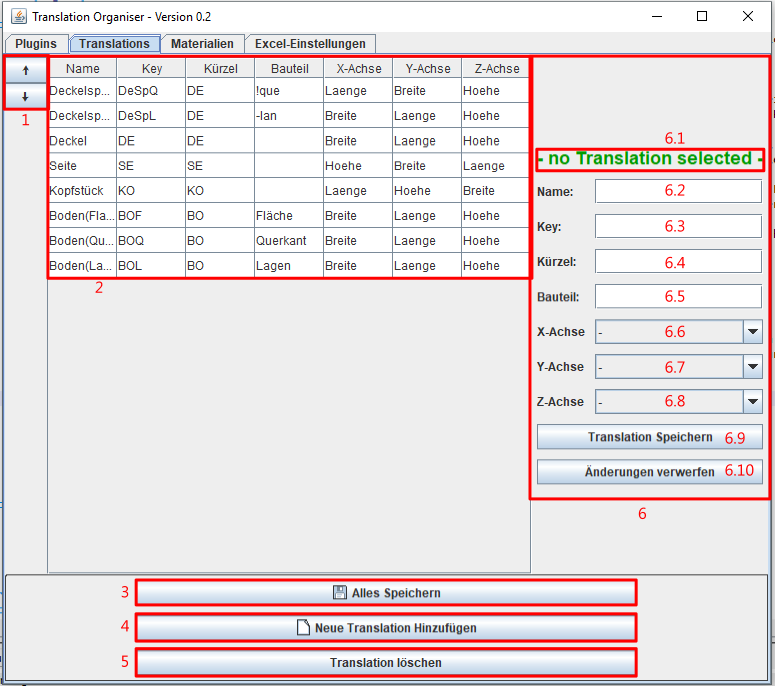
\includegraphics[scale=0.48]{pics/assisttool/translations-normal.png}
					\caption{Das Interface für Translations. \newline (Trotz älterer Version gültig)}
					\label{fig:translations normal}
				\end{figure}
				\begin{enumerate}
					\item Diese beiden Schaltflächen werden genutzt um eine Translation nach oben/unten zu bewegen und somit die Reihenfolge zu ändern. Bei der Reihenfolge wird es als früher interpretiert je weiter es oben ist.
					\item In dieser Tabelle werden Translations angezeigt mit den jeweiligen Eigenschaften für die verschiedenen Spalten. Ein Element kann durch einfaches anklicken angewählt werden für mögliche Reihenfolgen Änderungen (siehe 1.). Durch doppeltes anklicken gelangt man in den Bearbeitungsmodus. Mehr dazu unter \hyperref[translation-bearbeiten]{\ref{translation-bearbeiten}}.
					\item Diese Schaltfläche speichert alle Translations in einer Datei, welche dann von dem \robersexcelconvert-Plugin gelesen und verarbeitet wird.
					\hinweis{In der Version v0.2 muss man anschließend \sketchup neu starten um die Änderungen zu übernehmen}
					\item Diese Schaltfläche wird genutzt um eine neue Translation zu erzeugen. Mehr dazu unter \hyperref[translation-hinzufuegen]{\ref{translation-hinzufuegen}}.
					\item Diese Schaltfläche wird genutzt um eine vorhandene Translation zu löschen. Mehr dazu unter \hyperref[translation-loeschen]{\ref{translation-loeschen}}.
					\item Diese Sammlung von Elementen zeigt eine ausgewählte Translation an. Sie wird für sowohl das Bearbeiten als auch für das Hinzufügen von Translations genutzt. Sie unterteilt sich in:	
						\begin{enumerate}[label*=\arabic*]
							\item Der derzeitige Status. Es zeigt entweder wie im Beispiel \glqq\green{- no Translation selected -} \grqq, falls keine Translation derzeit bearbeitet wird, oder \glqq \red{Editing: NAME} \grqq für denn Fall, dass die Translation mit Kürzel NAME derzeit bearbeitet wird. 
							\item Der Name der aktuellen Translation
							\item Der Key der aktuellen Translation
							\item Das Kürzel der aktuellen Translation
							\item Das Bauteil der aktuellen Translation
							\item Die auf der X-Achse abgetragene Einheit
							\item Die auf der Y-Achse abgetragene Einheit
							\item Die auf der Z-Achse abgetragene Einheit
							\item Schaltfläche zum Speichern der Änderungen
							\item Schaltfläche um alle Änderungen zu verwerfen
						\end{enumerate}
				\end{enumerate}
			
			\subsection{Hinzufügen} \label{translation-hinzufuegen}
				Um eine Translation hinzuzufügen kann die in \hyperref[fig:translations normal]{\ref{fig:translations normal}} mit 4 bezeichnete Schaltfläche genutzt werden. Dies lädt in die mit 6 bezeichnete Gruppierung eine neue Translation.
				\hinweis{In der Version v0.2 werden die Elemente mit \glqq TESTName\grqq\xspace beschriftet.}
				Die Werte können bearbeitet und die neuen Daten eingetragen werden. Am Ende wird durch das betätigen der Schaltfläche 6.9 die neue Translation gespeichert. Falls das Kürzel bereits so verwendet wird erscheint eine Fehlermeldung und die Werte können weiter bearbeitet werden.
				\hinweis{Ein Test auf die beste Reihenfolge für das Bauteil wird in Version v0.2 nicht gemacht}
				Falls man die Translation nicht erstellen möchte kann man auch mittels 6.10 die Eingaben verwerfen.
				
			\subsection{Bearbeiten} \label{translation-bearbeiten}
				Um eine Translation zu bearbeiten kann die zu bearbeitende Translation per Doppelklick in der in \hyperref[fig:translations normal]{\ref{fig:translations normal}} mit 6 bezeichneten Gruppierung geladen werden. Das mit 6.1 bezeichnete Informationsfeld ändert sich dem entsprechend. Nach dem Bearbeiten kann analog zum Hinzufügen die Änderung gespeichert oder verworfen werden.
			\subsection{Löschen} \label{translation-loeschen}
				Um eine Translation zu löschen muss die durch einen einfach Klick angewählt werden und anschließend mittel der in \hyperref[fig:translations normal]{\ref{fig:translations normal}} mit 5 bezeichneten Schaltfläche gelöscht werden.
				\hinweis{In der Version v0.2 gibt es keine Nachfrage bzgl. des expliziten Wunsches}			
		\section{Materialien}\label{Material}
			Die Materialien bestimmten, welche Elemente im laufe der Transformation an zugewiesenen Oberflächen die Material-Texturen bekommen. Die Materialien können aber müssen nicht auf jeder Seite eine unterschiedliche Textur haben. Eine sogenannte Zuweisung wird innerhalb der Programme \glqq Material Assignment\grqq (Material Zuweisung) genannt. Eine solche Zuweisung hat den folgenden Aufbau:
				\begin{itemize}
					\setlength{\itemindent}{1cm}
					\item[Name:] Der Name, welcher für die Zuweisung verwendet werden soll. Er dient allein der Leserlichkeit bei Ausgaben
					\item[Key:] Der Key, welcher genutzt wird um eine Zuweisung innerhalb der Datei eindeutig zu identifizieren. Keine zwei Zuweisungen dürfen den selben Key haben.					
					\item[Materialgruppe:] Die Materialgruppe ist der erste Schritt der Identifizierung basierend auf der \glqq Materialgruppe\grqq-Spalte in der Excel-Datei. 
					\item[Werkstoff:] Der Werkstoff ist der zweite Schritt der Identifizierung. Analog zum Bauteil der Translations wird eine Zuweisung als geeignet anerkannt, falls sie die unter Werkstoff genannte Zeichenkette beinhaltet.
					\hinweis{Falls diese Spalte für eine Zelle leer ist, können alle Zuweisungen, welche das zugehörige Kürzel haben als geeignet angesehen}
					\item Die Restlichen Spalten namens: Vorne, Hinten, Links, Rechts, Oben, Unten definieren die Material-Texturen, welche den jeweiligen Seiten des zu erstellenden Rechtecks zugeordnet werden.
				\end{itemize}
			
			Das Material Zuweisungs-Interface besteht aus den folgenden Elementen, dargestellt in \hyperref[fig:materials-normal]{Fig. \ref{fig:materials-normal}}:
			\begin{figure}
				\centering
				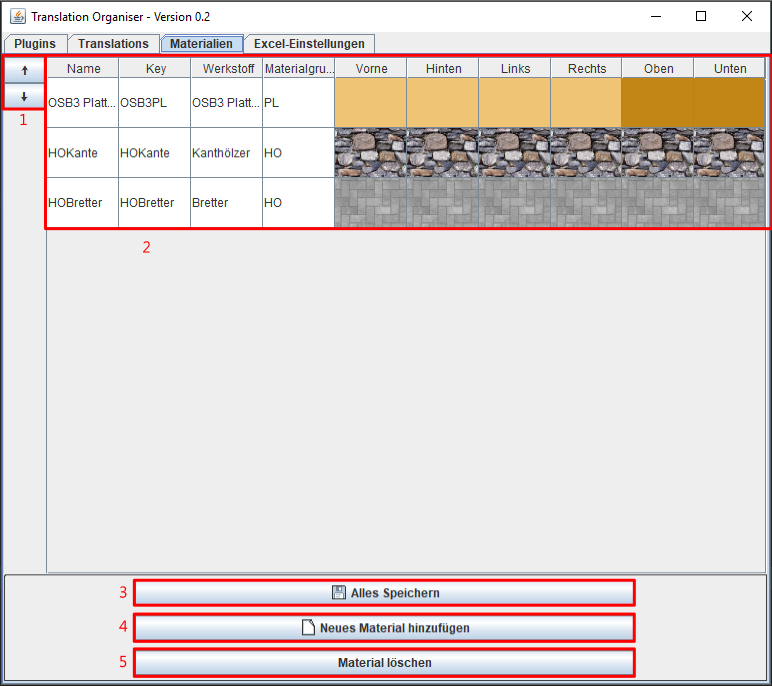
\includegraphics[scale=0.48]{pics/assisttool/materials-normal.png}
				\caption{Die Elemente des Material Zuweisungs-Interface\newline (Trotz älterer Version gültig)}
				\label{fig:materials-normal}
			\end{figure}
			
			\begin{enumerate}
				\item Diese beiden Schaltflächen werden genutzt um eine Zuweisung nach oben/unten zu bewegen und somit die Reihenfolge zu ändern. Bei der Reihenfolge wird es als früher interpretiert je weiter es oben ist.
				\item In dieser Tabelle werden die Zuweisungen angezeigt mit den jeweiligen Eigenschaften und Elementen in den jeweiligen Spalten.
				\item Diese Schaltfläche speichert alle Zuweisungen in einer Datei, welche dann von dem \robersexcelconvert-Plugin gelesen und verarbeitet wird.
				\hinweis{In der Version v0.2 muss man anschließend \sketchup neu starten um die Änderungen zu übernehmen}
				\item Diese Schaltfläche wird genutzt um eine neue Translation zu erzeugen. Mehr dazu unter \ref{material-hinzufuegen}.
				\item Diese Schaltfläche wird genutzt um eine vorhandene Translation zu löschen. Mehr dazu unter \hyperref[material-loeschen]{\ref{material-loeschen}}.
			\end{enumerate}
		
			\subsection{Hinzufügen}	\label{material-hinzufuegen}		
				\begin{wrapfigure}[12]{r}{0.4\textwidth}
					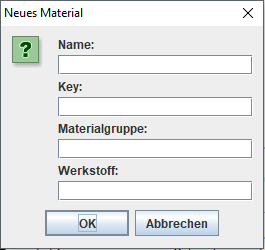
\includegraphics[scale=0.48]{pics/assisttool/materials-add.PNG}
					\caption{Der Dialog um ein Material hinzuzufügen}
					\label{fig:materials add}
				\end{wrapfigure}
				Um eine neue Material Zuweisung hinzuzufügen kann die unter \hyperref[fig:materials-normal]{Fig. \ref{fig:materials-normal}} bezeichnete 4 genutzt werden. Diese öffnet den Eingabe-Dialog aus \hyperref[fig:materials add]{Abbildung \ref{fig:materials add}}. Dort müssen der Name, Key, Materialgruppe und Werkstoff eingegeben werden. 
				\hinweis{In Version v0.2 gibt es noch keine Überprüfung bezüglich Wählbarkeit und null-werte}
				Als Materialien wird auf jeder Seite das erste dem Programm bekannte Material genommen.
				\hinweis{Für weitere Versionen ist ein Default-Material einzufügen}
			\subsection{Bearbeiten}
				
				Um eine Zuweisung zu bearbeiten müssen zwei Sachen unterschieden werden.
				\begin{wrapfigure}[20]{r}{0.4\textwidth}
					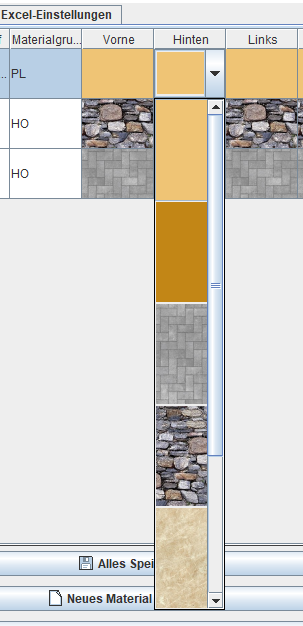
\includegraphics[scale=0.48]{pics/assisttool/materials-dropdown.PNG}
					\caption{Das Ändern eines Materials}
					\label{fig:materials aendern}
				\end{wrapfigure}
				\subsubsection*{Ändern von: Name, Key, Materialgruppe, Werkstoff}
					Diese Elemente können geändert werden durch eine Doppelklick auf die jeweilige Zelle der zu ändernden Zuweisung und das manuelle Eintippen des neuen Wertes.
					\hinweis{In Version v0.2 gibt es keine Überprüfung bzgl. der Verfügbarkeit von z.B. Keys}
				\subsubsection*{Ändern eines Materials}
					
					Um ein Material zu ändern kann man auf die jeweilige Zelle der Zuweisung klicken. Dort öffnet sich dann ein Dropdown Menu zusehen in \hyperref[fig:materials aendern]{Abbildung \ref{fig:materials aendern}}. Die wählbaren Materialien sind dort aufgelistet. \\
					Ein Material, normalerweise das letzte Material, ist das sogenannte Fehler Material. Dieses wird Oberflächen gegeben, für die die Textur fehlt (siehe \hyperref[semantic check]{\ref{semantic check}}). Diese sollte für keine weitere Fläche verwendet werden.
			\subsection{Löschen} \label{material-loeschen}
				Um eine Material Zuweisung zu löschen kann diese durch einfach Klick angewählt und durch die in \hyperref[fig:materials-normal]{Fig. \ref{fig:materials-normal}} mit 5 gezeichnete Schaltfläche gelöscht werden.
	 			\hinweis{In der Version v0.2 gibt es keine Nachfrage bzgl. des expliziten Wunsches}			
	 	\section{Excel Konstanten}\label{excel konstanten}
			 Um die unter \ref{excel} genannten Werte für die Zeilen und Spalten innerhalb der Excel-Datei zu ändern bietet das \assisttool einen Reiter mit einem Interface für eben jene Aufgabe. Mit den Standartwerten ist das Interface in \hyperref[fig:excel constants]{Abbildung \ref{fig:excel constants}} gegeben.
		 	\begin{figure}[H]
		 		\centering
		 		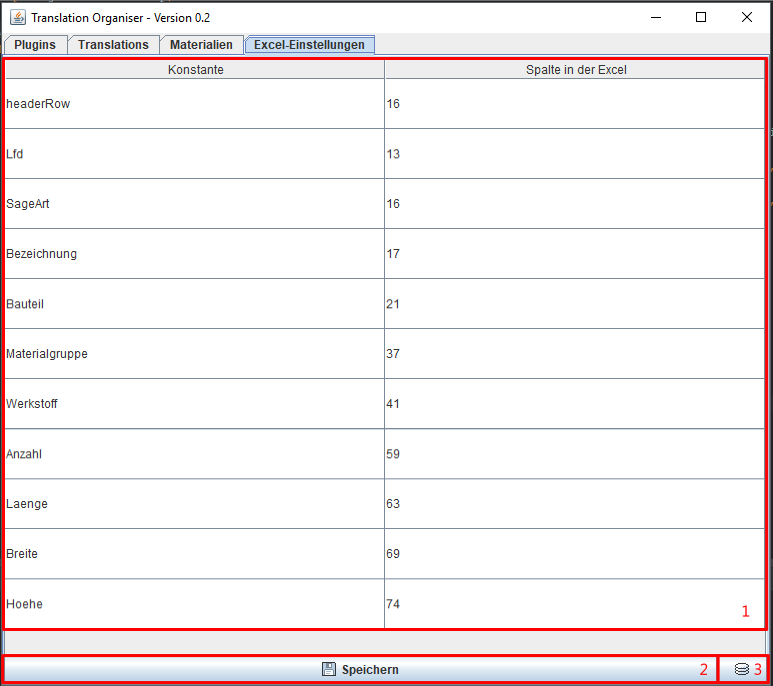
\includegraphics[scale=0.48]{pics/assisttool/excel-konstanten.PNG}
		 		\caption{Das Excel Konstanten Bearbeitungs-Interface\newline (Trotz älterer Version gültig)}
		 		\label{fig:excel constants}
		 	\end{figure}
		 	Das Interface unterteilt sich in 3 Komponenten:
			 	\begin{enumerate}
			 		\item Die Tabelle mit den Konstanten mit den selben Namen wie sie im Code auftreten
			 		\item Eine Schaltfläche um vorgenommene Änderungen zu speichern
			 		\item Eine Schaltfläche um die zugrundeliegende Datei neu einzulesen
			 	\end{enumerate}
		 	
		 	Um eine Zeile zu ändern kann die entsprechende Zelle per Doppelklick bearbeitet werden.
		 	\hinweis{In Version v0.2 gibt es keine Überprüfung bzgl. der Werte}
	 	
	\chapter{Excel-Datei}\label{excel}
		Die Excel-Datei ist die Eingabe, welche der \assisttool bekommt. Alles weitere basiert auf den Werten der einzelnen Einträge an bestimmten Stellen. Das einzige sogenannte \glqq Worksheet \grqq, welches während der Verarbeitung genutzt wird trägt den Namen \glqq Dimensionsware \grqq, zusehen in \hyperref[fig:dimensionsware worksheet]{Abbildung \ref{fig:dimensionsware worksheet}}.		
		\begin{figure}[H]
			\centering
			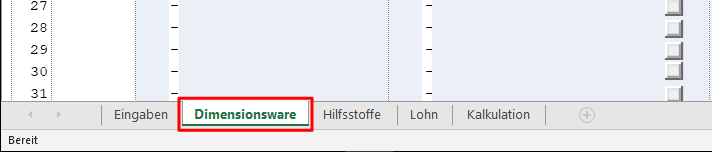
\includegraphics[scale=0.48]{pics/excel/reiter_auswaehlen.png}
			\caption{Das benötigte \glqq Worksheet \grqq}
			\label{fig:dimensionsware worksheet}
		\end{figure}
		
		\section{Aufbau}
			Der Aufbau der Excel folgt einer bestimmten Ordnung. Es müssen die Elemente in tabellarisch angeordnet sein um ein auslesen zu ermöglichen. Dabei entspricht einer Zeile genau einem Element, welches dann durch die Translations identifiziert wird und durch die Material Zuweisungen die Texturen erhält. \\
			Der Aufbau der Datei erfolgt in Version v1.1 nach dem in \hyperref[fig:excel file]{Abbildung \ref{fig:excel file}} dargestellten Schema.
			
			\begin{figure}[H]
				\centering
				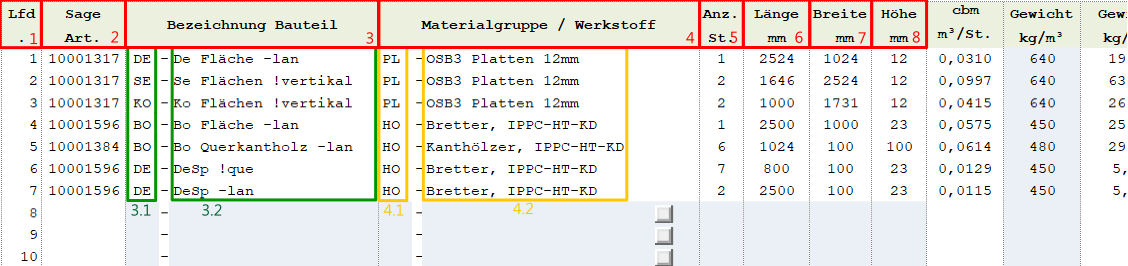
\includegraphics[scale=0.48]{pics/excel/dimensionsware.png}
				\caption{Aufbau der Excel Datei}
				\label{fig:excel file}
			\end{figure}
		
			Die Eigenschaften eines Elementes unterteilen sich in den Tabellen-Header und den Tabellen Rumpf. Falls ein Tabellen-Header genau eine Eigenschaft definiert sind die Spalte des Headers und der Eigenschaft gleich. Bei Tabellen-Headern, wie z.B. \glqq Bezeichnung Baumaterial \grqq (3) unterteilt sich jede Zelle darunter in die Eigenschaften \glqq Bezeichnung \grqq (3.1) und \glqq Bauteil \grqq (3.2). Diese haben jeweils eine andere zugrundeliegende Spalte in der Excel-Datei.\\
			
			Die Standartwerte der Spalten ist gegeben in \hyperref[tab:columnvalues]{Abbildung \ref{tab:columnvalues}}.\\
			\begin{figure}[H]
				\begin{tabular}{c|l|l | l | l}
					Nummer & Tabellen-Header & Spalte & Eigenschaft & erwartete Werte \\ \hline \hline
					1 & Lfd.& 13 & - & Integer($>0$) \\
					2 & Sage Art. & 16 & - & Integer \\
					3.1 & Bezeichnung Bauteil & 17 & Bezeichnung & String \\
					3.2 & Bezeichnung Bauteil & 21 & Bauteil & String \\
					4.1 & Materialgruppe/Werkstoff & Materialgruppe & 37 & String \\
					4.1 & Materialgruppe/Werkstoff & Werkstoff & 41 & String \\
					5 & Anzahl & 59 & Anzahl & Integer($>0$)\\
					6 & Länge & 63 & Laenge &  Integer(mm) \\
					7 & Breite & 69 & Breite & Integer(mm) \\
					8 & Höhe & 74 & Hoehe & Integer(mm) \\
					9 &  & 161 & KoordinatenStart & Integer (>0)
				\end{tabular}
				\caption{Standartwerte der Spalten für die verschiedenen Elemente}
				\label{tab:columnvalues}
			\end{figure}
			
			Dabei spielen der Werte \glqq Lfd.\grqq nur eine Rolle für den Semantik-Check. Die Spalte von \glqq Sage Art. \grqq wird hingegen verwendet um zu ermitteln wie viele Elemente in der Liste vorhanden sind. Sobald diese Spalte für eine Zeile keinen Wert hat, wir dort der Punkt gesetzt hinter welchem keine weiteren Elemente gesucht werden.\\						
			Zudem gibt es einen Wert, welcher die Zeile definiert in welcher der Header steht. Diese hat standardmäßig den Wert 16. Wird dieser angepasst, so wird der Semantik-Check der Excel dementsprechend auf eine andere Zeile verschoben. Die Spalten bleiben dabei gleich. Um die Spalten und Zeile anzupassen siehe \ref{excel konstanten}.
		\subsection{Koordinaten}
			Ab Version v1.1 werden die Koordinaten für die Elemente, welche als Kiste gebaut werden sollen, ebenfalls in der Excel gespeichert. Eine Beispiel-Abbildung von Koordinaten ist zu sehen in Abbildung \ref{fig:koordinaten}. Falls kein Wert gefunden wird wird per default eine 0 als Wert genommen.
			\begin{figure}
				\centering
				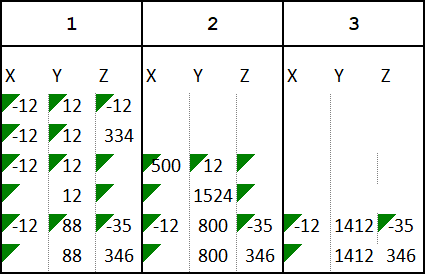
\includegraphics[scale=0.48]{pics/excel/koordinaten.png}
				\caption{Die Koordinaten innerhalb der Excel-Datei}
				\label{fig:koordinaten}
			\end{figure}
			Die Koordinaten werden wie in \ref{element bearbeiten} beschrieben bei der unteren linken Ecke gewählt.
	\chapter{Beispiele}
		
\end{document}